% !TEX TS-program = pdflatex
% !TEX encoding = UTF-8 Unicode

% This is a simple template for a LaTeX document using the "article" class.
% See "book", "report", "letter" for other types of document.

\documentclass[11pt]{article} % use larger type; default would be 10pt

\usepackage[utf8]{inputenc} % set input encoding (not needed with XeLaTeX)
\usepackage{float} % para que las imagenes no se metan donde se les canta el orto

%%% Examples of Article customizations
% These packages are optional, depending whether you want the features they provide.
% See the LaTeX Companion or other references for full information.

%%% PAGE DIMENSIONS
\usepackage[top=3cm]{geometry} % to change the page dimensions
\geometry{a4paper} % or letterpaper (US) or a5paper or....
% \geometry{margin=2in} % for example, change the margins to 2 inches all round
% \geometry{landscape} % set up the page for landscape
%   read geometry.pdf for detailed page layout information

\usepackage{graphicx} % support the \includegraphics command and options

% \usepackage[parfill]{parskip} % Activate to begin paragraphs with an empty line rather than an indent

%%% PACKAGES
\usepackage[spanish]{babel} % para que el documento sea en argentino y de bokita el mas grande papá
\usepackage{booktabs} % for much better looking tables
\usepackage{array} % for better arrays (eg matrices) in maths
\usepackage{paralist} % very flexible & customisable lists (eg. enumerate/itemize, etc.)
\usepackage{verbatim} % adds environment for commenting out blocks of text & for better verbatim
\usepackage{subfig} % make it possible to include more than one captioned figure/table in a single float
% These packages are all incorporated in the memoir class to one degree or another...

%%% HEADERS & FOOTERS
\usepackage{fancyhdr} % This should be set AFTER setting up the page geometry
\pagestyle{fancy} % options: empty , plain , fancy
\renewcommand{\headrulewidth}{0pt} % customise the layout...
\lhead{}\chead{}\rhead{}
\lfoot{}\cfoot{\thepage}\rfoot{}

%%% SECTION TITLE APPEARANCE
\usepackage{sectsty}
\allsectionsfont{\sffamily\mdseries\upshape} % (See the fntguide.pdf for font help)
% (This matches ConTeXt defaults)

%%% ToC (table of contents) APPEARANCE
\usepackage[nottoc,notlof,notlot]{tocbibind} % Put the bibliography in the ToC
\usepackage[titles,subfigure]{tocloft} % Alter the style of the Table of Contents
\renewcommand{\cftsecfont}{\rmfamily\mdseries\upshape}
\renewcommand{\cftsecpagefont}{\rmfamily\mdseries\upshape} % No bold!

%%% END Article customizations

%%% The "real" document content comes below...

\title{Práctica/Laboratorio de IPv4 (1)}
\author{Amoroso, Lihuel Pablo 13497/2; Gasquez, Federico Ramón 13598/6}
\date{Grupo A} % Activate to display a given date or no date (if empty),
         % otherwise the current date is printed 

\begin{document}
    \maketitle

    \section{Utilizando la topología topologia-IP.imn y dado el bloque IPv4 asignado resolver:}

    \begin{figure}[htbp]
        \centering
        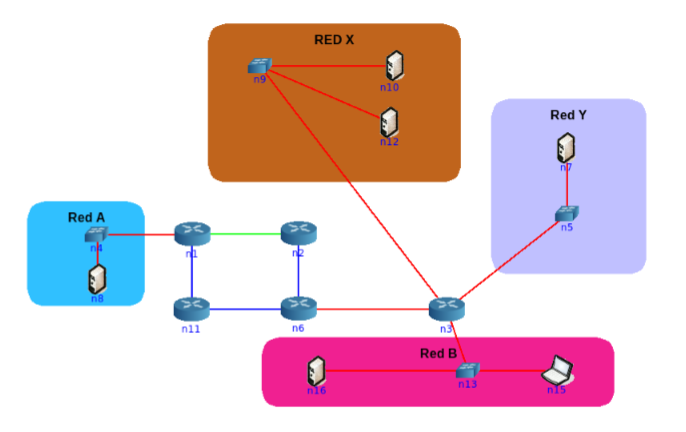
\includegraphics[]{topologia.png}
        \caption{Esquema a subnetear}
        \label{fig:topologia}
    \end{figure}

        \subsection{Arme el plan de direccionamiento IPv4 teniendo en cuenta las siguientes restricciones:}
        \begin{itemize}
            \item La red A tiene 70 hosts y se espera un crecimiento máximo de 20 hosts.
            \item La red X tiene 150 hosts.
            \item La red B cuenta con 20 hosts.
            \item La red Y tiene 35 hosts y se espera un crecimiento máximo de 30 hosts.
            \item Los bloques IP asignados en los enlaces entre routers podrán ajustarse a desperdiciar pocas direcciones.
            \item ¿Es importante utilizar VLSM?

                Si, ya que de esa manera se desperdician menos direcciones.
        \end{itemize}

        \subsection{Asigne direcciones IP en los equipos de la topología según el plan anterior.}
        
        \paragraph{Si bien se adjunta la topología de forma que se pueda efectivamente verificar que las direcciones han sido correctamente asignadas, se procederá a detallar el procedimiento utilizado.}
        \paragraph{Primero ha de determinarse la red con más hosts. Esto se realiza para poder determinar cuántos bits se utilizarán como máximo. En este caso, la red con más hosts es la red X con 150.}
        \paragraph{De ahí, los pasos a seguir para asignar direcciones IP a los equipos en la topología se pueden reducir en los siguientes:}
        \begin{itemize}
            \item Determinar la red con más cantidad de hosts.
            \item Usar una de las redes sobrantes para subnetear.
            \item Determinar cuáles son las redes sobrantes para el próximo subnet(si hubiera).
        \end{itemize}
        \paragraph{Aplicando el concepto al problema, tenemos la dirección 51.37.192.0/19. La red con más hosts, como ya se concluyó antes, es la red X con 150 hosts. Para representar tal cantidad, son necesarios 8 bits(con 7 bits, hay 24 hosts que se me quedan afuera) con un desperdicio de 104 hosts. Como voy a usar 8 bits, voy a correr la máscara a 24 en lugar de dejarla en 19. Concluyendo, la dirección que se asignará a la red X será la 51.37.192.0/24. Sobrarán, de esta forma, 32 direcciones de red y la siguiente a la asignada a la red X(51.37.193.0/24) será la próxima a subnetear.}
        \paragraph{Habiéndole asignado una dirección a la red X, la red con más hosts ahora es la red A con 90 hosts. Para representar tal cantidad, son necesarios 7 bits(con 6 bits, hay 28 hosts que se me quedan afuera) con un desperdicio de 36 hosts. Como voy a usar 7 bits, voy a correr la máscara a 25 en lugar de dejarla en 24. Concluyendo, la dirección que se asignará a la red A será la 51.37.193.0/25. Sobrará, de este modo, 1 dirección de red(51.37.193.128/25) que será la próxima a subnetear.}
        \paragraph{Habiéndole asignado una dirección a la red X y A, la red con más hosts es ahora la red Y con 65 hosts. Para representar tal cantidad, son necesarios 7 bits(con 6 bits, hay 3 hosts que se me quedan afuera) con un desperdicio de 61 hosts. Como voy a usar 7 bits, la máscara queda intacta(en /25). Concluyendo, la dirección que se asignará a la red Y será la 51.37.193.128/25. En este caso, no sobran más direcciones, por lo que será necesario tomar la siguiente a la siguiente de la red A(51.37.194.0/24) y será ésta la próxima a subnetear.}
        \paragraph{Habiéndole asignado una dirección a la red X, A y Y, la red con más hosts ahora(y la última que resta) es la red B con 20 hosts. Para representar tal cantidad, son necesarios 5 bits(con 4 bits, hay 6 hosts que se me quedan afuera) con un desperdicio de 10 hosts. Como voy a usar 5 bits, voy a correr la máscara a 27 en lugar de dejarla en 24. Concluyendo, la dirección que se asignará a la red B será la 51.37.194.0/27. Sobrarán, así, 7 direcciones de red y la siguiente a la asignada a la red B(51.37.194.32/27)será la próxima a subnetear.}
        \paragraph{Habiéndose ya asignado una dirección a las redes principales(red A, B, X e Y), es que ahora toca asignar direcciones a los enlaces punto a punto. Para asignar direcciones IP punto a punto débese tener en cuenta que solo son necesarios 4 hosts: el host reservado, el extremo A, el extremo B y el host de broadcast. Por esto es que serán necesarios 2 bits(con 1 bit, hay dos hosts que se me quedan afuera) para tal representación. Así mismo, existen 5 enlaces punto a punto: n1-n2, n1-n11, n2-n6, n6-n11 y n6-n3, por lo que se necesitan 3 bits(con 2 bits, hay 1 enlace punto a punto que no puedo representar) con un desperdicio de 3 redes. Teniendo la dirección 51.37.194.32/27, voy a correr la máscara de 27 a 30, indicando que solo utilizaré 4 hosts. De 27 a 30 hay 3, es decir, hay 3 bits que podré utilizar como redes a enlaces punto a punto, esto es, podré asignar 8 redes. Son necesarias 5 redes para los enlaces punto a punto, por lo que puedo continuar(podría haber pasado que no hubieran suficientes bits para representar las redes punto a punto. En tal caso hubiera sido necesario usar la dirección siguiente a la siguiente a la siguiente de la red A, es decir, la 51.37.195.0/24). Concluyendo, asignaré la red 51.37.194.32/30 al enlace n1-n2, 51.37.194.36/30 al enlace n1-n11, 51.37.194.40/30 al enlace n2-n6, 51.37.194.44/30 al enlace n6-n11 y 51.37.194.48/30 al enlace n6-n3.}
        \paragraph{Pasando en limpio(y agregando las direcciones asignadas a los hosts):}
        \begin{itemize}
            \item Red X: 51.37.192.0/24.
            \begin{itemize}
                \item n3(router-eth2): 51.37.192.1/24.
                \item n10(host-eth0): 51.37.192.2/24.
                \item n12(host-eth0): 51.37.192.3/24.
            \end{itemize}
            \item Red A: 51.37.193.0/25.
            \begin{itemize}
                \item n1(router-eth0): 51.37.193.1/25.
                \item n8(host-eth0): 51.37.193.2/25.
            \end{itemize}
            \item Red Y: 51.37.193.128/25.
            \begin{itemize}
                \item n3(router-eth1): 51.37.193.129/25.
                \item n7(host-eth0): 51.37.193.130/25.
            \end{itemize}
            \item Red B: 51.37.194.0/27.
            \begin{itemize}
                \item n3(router-eth3): 51.37.194.1/27.
                \item n15(host-eth0): 51.37.194.2/27.
                \item dhcp-server(host-eth0): 51.37.194.3/27.
            \end{itemize}
            \item Enlace punto-a-punto n1-n2: 51.37.194.32/30.
            \begin{itemize}
                \item n1(router-eth1): 51.37.194.33/30.
                \item n2(router-eth0): 51.37.194.34/30.
            \end{itemize}
            \item Enlace punto-a-punto n1-n11: 51.37.194.36/30.
            \begin{itemize}
                \item n1(router-eth2): 51.37.194.37/30.
                \item n11(router-eth0): 51.37.194.38/30.
            \end{itemize}
            \item Enlace punto-a-punto n2-n6: 51.37.194.40/30.
            \begin{itemize}
                \item n2(router-eth1): 51.37.194.41/30.
                \item n6(router-eth0): 51.37.194.42/30.
            \end{itemize}
            \item Enlace punto-a-punto n6-n11: 51.37.194.44/30.
            \begin{itemize}
                \item n6(router-eth2): 51.37.194.45/30.
                \item n11(router-eth1): 51.37.194.46/30.
            \end{itemize}
            \item Enlace punto-a-punto n6-n3: 51.37.194.48/30.
            \begin{itemize}
                \item n6(router-eth1): 51.37.194.49/30.
                \item n3(router-eth0): 51.37.194.50/30.
            \end{itemize}
        \end{itemize}

        \subsection{Configure las tablas de rutas teniendo en cuenta que n1 deberá optar por el enlace verde solamente para rutear el tráfico dirigido a la Red X.}  

        \begin{itemize}
            \item n8

            \begin{tabular}{ |c|c|c|c| } 
            \hline
                Destination & Gateway & GenMask & Iface \\
            \hline
                0.0.0.0 & 51.37.193.1 & 0.0.0.0 & eth0 \\
            \hline
            \end{tabular}
            \item n1
            
            \begin{tabular}{ |c|c|c|c| } 
            \hline
                Destination & Gateway & GenMask & Iface \\
            \hline
                51.37.192.0 & 51.37.194.34 & 255.255.255.0 & eth1 \\
                51.37.193.0 & 0.0.0.0 & 255.255.255.128 & eth0 \\
                51.37.193.128 & 51.37.194.38 & 255.255.255.128 & eth0 \\
                51.37.194.0 & 51.37.194.38 & 255.255.255.224 & eth2 \\
                51.37.194.32 & 0.0.0.0 & 255.255.255.252 & eth1 \\
                51.37.194.36 & 0.0.0.0 & 255.255.255.252 & eth2 \\
                51.37.194.40 & 51.37.194.34 & 255.255.255.252 & eth1 \\
                51.37.194.44 & 51.37.194.38 & 255.255.255.252 & eth2 \\
                51.37.194.48 & 51.37.194.38 & 255.255.255.252 & eth2 \\
            \hline
            \end{tabular}
            \item n11
            
            \begin{tabular}{ |c|c|c|c| } 
            \hline
                Destination & Gateway & GenMask & Iface \\
            \hline
                51.37.192.0 & 51.37.194.46 & 255.255.255.0 & aaa \\
                51.37.193.0 & 51.37.194.37 & 255.255.255.128 & eth0 \\
                51.37.193.128 & 51.37.194.45 & 255.255.255.128 & eth0 \\
                51.37.194.0 & 51.37.194.45 & 255.255.255.224 & eth2 \\
                51.37.194.32 & 51.37.194.37 & 255.255.255.252 & eth1 \\
                51.37.194.36 & 0.0.0.0 & 255.255.255.252 & eth2 \\
                51.37.194.40 & 51.37.194.45 & 255.255.255.252 & eth1 \\
                51.37.194.44 & 0.0.0.0 & 255.255.255.252 & eth2 \\
                51.37.194.48 & 51.37.194.45 & 255.255.255.252 & eth2 \\
            \hline
            \end{tabular}
            \item n2
            
            \begin{tabular}{ |c|c|c|c| } 
            \hline
                Destination & Gateway & GenMask & Iface \\
            \hline
                51.37.192.0 & 51.37.194.42 & 255.255.255.0 & aaa \\
                51.37.193.0 & 51.37.194.33 & 255.255.255.128 & eth0 \\
                51.37.193.128 & 51.37.194.42 & 255.255.255.128 & eth0 \\
                51.37.194.0 & 51.37.194.42 & 255.255.255.224 & eth2 \\
                51.37.194.32 & 0.0.0.0 & 255.255.255.252 & eth1 \\
                51.37.194.36 & 51.37.194.33 & 255.255.255.252 & eth2 \\
                51.37.194.40 & 0.0.0.0 & 255.255.255.252 & eth1 \\
                51.37.194.44 & 51.37.194.42 & 255.255.255.252 & eth2 \\
                51.37.194.48 & 51.37.194.42 & 255.255.255.252 & eth2 \\
            \hline
            \end{tabular}
            \item n6
            
            \begin{tabular}{ |c|c|c|c| } 
            \hline
                Destination & Gateway & GenMask & Iface \\
            \hline
                51.37.192.0 & 51.37.194.50 & 255.255.255.0 & aaa \\
                51.37.193.0 & 51.37.194.41 & 255.255.255.128 & eth0 \\
                51.37.193.128 & 51.37.194.42 & 255.255.255.128 & eth0 \\
                51.37.194.0 & 51.37.194.50 & 255.255.255.224 & eth2 \\
                51.37.194.32 & 51.37.194.41 & 255.255.255.252 & eth1 \\
                51.37.194.36 & 51.37.194.46 & 255.255.255.252 & eth2 \\
                51.37.194.40 & 0.0.0.0 & 255.255.255.252 & eth1 \\
                51.37.194.44 & 0.0.0.0 & 255.255.255.252 & eth2 \\
                51.37.194.48 & 0.0.0.0 & 255.255.255.252 & eth2 \\
            \hline
            \end{tabular}
            \item n3
            
            \begin{tabular}{ |c|c|c|c| } 
            \hline
                Destination & Gateway & GenMask & Iface \\
            \hline
                51.37.192.0 & 0.0.0.0 & 255.255.255.0 & aaa \\
                51.37.193.0 & 51.37.194.49 & 255.255.255.128 & eth0 \\
                51.37.193.128 & 0.0.0.0 & 255.255.255.128 & eth0 \\
                51.37.194.0 & 0.0.0.0 & 255.255.255.224 & eth2 \\
                51.37.194.32 & 51.37.194.49 & 255.255.255.252 & eth1 \\
                51.37.194.36 & 51.37.194.49 & 255.255.255.252 & eth2 \\
                51.37.194.40 & 51.37.194.49 & 255.255.255.252 & eth1 \\
                51.37.194.44 & 51.37.194.49 & 255.255.255.252 & eth2 \\
                51.37.194.48 & 0.0.0.0 & 255.255.255.252 & eth2 \\
            \hline
            \end{tabular}
            \item n12

            \begin{tabular}{ |c|c|c|c| } 
            \hline
                Destination & Gateway & GenMask & Iface \\
            \hline
                0.0.0.0 & 51.37.192.1 & 0.0.0.0 & eth0 \\
            \hline
            \end{tabular}
            \item n10

            \begin{tabular}{ |c|c|c|c| } 
            \hline
                Destination & Gateway & GenMask & Iface \\
            \hline
                0.0.0.0 & 51.37.192.1 & 0.0.0.0 & eth0 \\
            \hline
            \end{tabular}
            \item n15

            \begin{tabular}{ |c|c|c|c| } 
            \hline
                Destination & Gateway & GenMask & Iface \\
            \hline
                0.0.0.0 & 51.37.194.1 & 0.0.0.0 & eth0 \\
            \hline
            \end{tabular}
            \item dhcp-server

            \begin{tabular}{ |c|c|c|c| } 
            \hline
                Destination & Gateway & GenMask & Iface \\
            \hline
                0.0.0.0 & 51.37.194.1 & 0.0.0.0 & eth0 \\
            \hline
            \end{tabular}
            \item n7

            \begin{tabular}{ |c|c|c|c| } 
            \hline
                Destination & Gateway & GenMask & Iface \\
            \hline
                0.0.0.0 & 51.37.193.129 & 0.0.0.0 & eth0 \\
            \hline
            \end{tabular}
        \end{itemize}

        \subsection{Utilizando la herramienta ping(8), verifique conectividad entre los hosts pertenecientes a las diferentes redes de usuarios.}

        \begin{figure}[htbp]
            \centering
            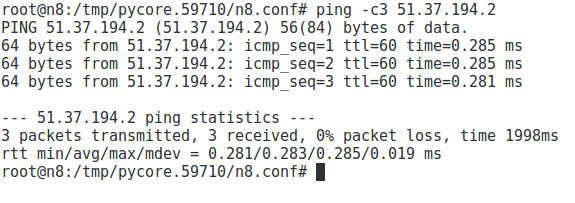
\includegraphics[]{ping_a-b.png}
            \caption{PING entre red A y red B}
            \label{fig:ping_a-b}
        \end{figure}
        \begin{figure}[htbp]
            \centering
            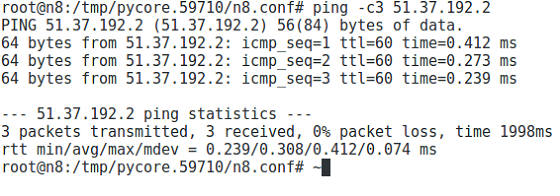
\includegraphics[]{ping_a-x.png}
            \caption{PING entre red A y red X}
            \label{fig:ping_a-x}
        \end{figure}
        \begin{figure}[htbp]
            \centering
            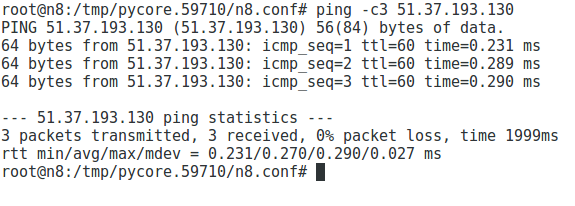
\includegraphics[]{ping_a-y.png}
            \caption{PING entre red A y red Y}
            \label{fig:ping_a-y}
        \end{figure}
        \begin{figure}[htbp]
            \centering
            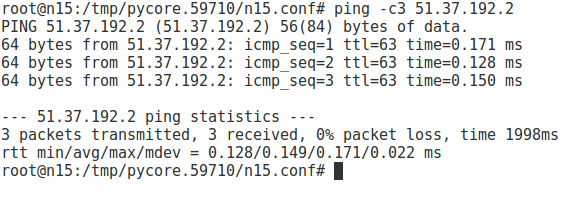
\includegraphics[]{ping_b-x.png}
            \caption{PING entre red B y red X}
            \label{fig:ping_b-x}
        \end{figure}
        \begin{figure}[htbp]
            \centering
            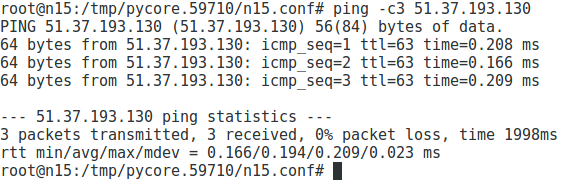
\includegraphics[]{ping_b-y.png}
            \caption{PING entre red B y red Y}
            \label{fig:ping_b-y}
        \end{figure}
        \begin{figure}[htbp]
            \centering
            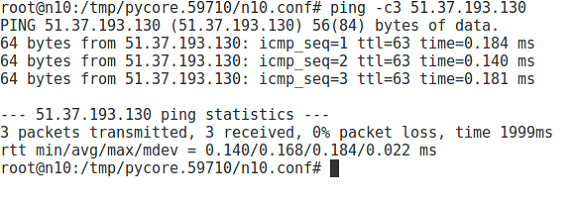
\includegraphics[]{ping_x-y.png}
            \caption{PING entre red X y red Y}
            \label{fig:ping_x-y}
        \end{figure}

    \section{TTL(Adjunte capturas de tráfico para cada uno de los incisos):}
        \subsection{Utilizando el comando traceroute(1)/mtr(8), realice una traza entre el host n8 y n10, tanto utilizando UDP como ICMP ¿Qué diferencias tiene cada método y en qué casos utilizaría cada uno?}

        \begin{figure}[htbp]
            \centering
            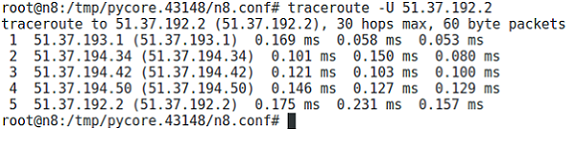
\includegraphics[]{traceroute_UDP_n8-n10.png}
            \caption{Traceroute usando UDP entre n8 y n10}
            \label{fig:traceroute_UDP_n8-n10}
        \end{figure}
        \begin{figure}[htbp]
            \centering
            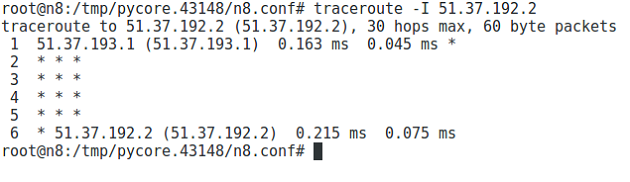
\includegraphics[]{traceroute_ICMP_n8-n10.png}
            \caption{Traceroute usando ICMP entre n8 y n10}
            \label{fig:traceroute_ICMP_n8-n10}
        \end{figure}
        \begin{figure}[H]
            \centering
            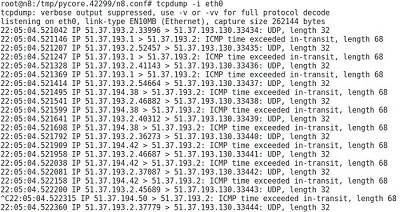
\includegraphics[]{tcpdump-eth0-ICMP.jpg}
            \caption{Como puede observarse, usando ICMP devuelve \textit{ICMP time exceeded}}
            \label{tcpdump-eth0-ICMP}
        \end{figure}

        \paragraph{Aplicando traceroute --icmp solo nos muestra el primer salto y la llegada al host destino. Aplicando traceroute --udp nos muestra todos los saltos intermedios hasta llegar al host destino.}
 
        \paragraph{La diferencia radica en la información que viene en el paquete de vuelta: en el caso de UDP el TTL vuelve expirado y en ICMP, HOST Unreachable.}
        
        \paragraph{En traceroute UDP, el cliente transmite a UDP un simple paquete a un valor de puerto de destino. Si el puerto es filtrado, devuelve HOST Unreachable. Por eso es que para estos casos es mejor usar ICMP.}

        \subsection{Realice un ping entre n8 y n5 y determine el valor inicial del campo TTL capturando tráfico en la interfaz eth0 del host n8.}

        \begin{figure}[H]
            \centering
            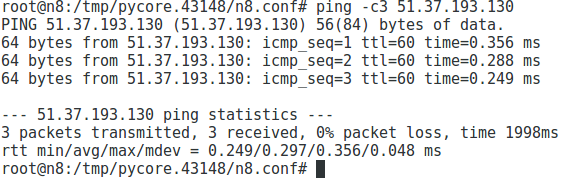
\includegraphics[]{ping_TTL_n8.png}
            \caption{PING entre n8 y n5}
            \label{fig:ping_TTL_n8.png}
        \end{figure}

        El valor inicial del TTL es 60.

        \subsection{A través de la capturas de tráfico, determine en qué momento el router decrementa el valor del TTL.}

        \begin{figure}[H]
            \centering
            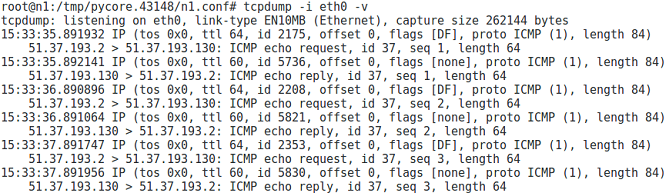
\includegraphics[]{tcpdump_TTL_n8_eth0.png}
            \caption{TCPdump que captura tráfico en la interfaz eth0}
            \label{fig:tcpdump_TTL_n8_eth01}
        \end{figure}
        \begin{figure}[H]
            \centering
            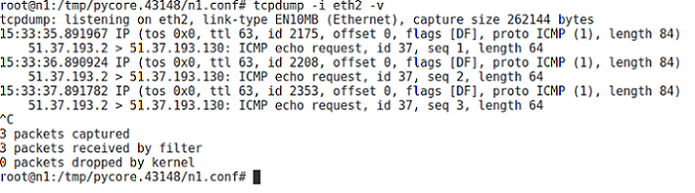
\includegraphics[]{tcpdump_TTL_n8_eth2.png}
            \caption{TCPdump que captura tráfico en la interfaz eth2}
            \label{fig:tcpdump_TTL_n8_eth2}
        \end{figure}

        Se puede observar en las diferentes capturas que por cada salto que hace el TTL se decrementa en 1: empieza en 64, luego hace un salto y se decrementa en 1 y pasa a 63. El TTL se decrementa tantas veces como hosts haya pasado.


        \subsection{Utilizando la herramienta para enviar mensajes ICMP con la opción -t desde n8 envíe un datagrama a n7 con TTL=1 ¿Qué mensaje recibe? ¿Por qué?}

        \begin{figure}[H]
            \centering
            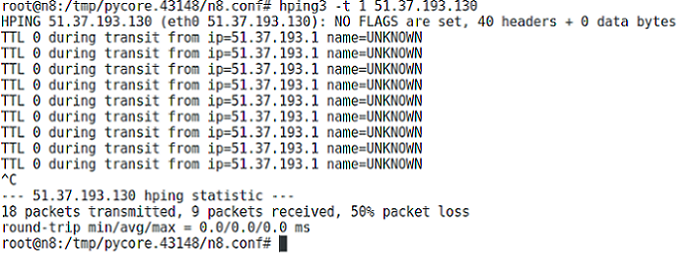
\includegraphics[]{hping3_TTL_n8.png}
            \caption{Envío del datagrama desde n8 a n7 usando hping3}
            \label{fig:hping3_TTL_n8}
        \end{figure}

        \paragraph{La respuesta nos dice que el TTL dio 0 antes de llegar al host(que es desconocido). Esto es porque el TTL se va decrementando en 1 cada vez que pasa por un host(router) y como lo configuramos en 1, el primer router lo decremento, este TTL quedó en 0 y por ende, el router lo devuelve con "tiempo de vida agotado".}

    \section{Fragmentación:}
        \subsection{Cambiando los MTU y enviando tráfico desde un host de la parte “A” a la “B” ver de forzar que los routers fragmenten.}

        \paragraph{Si bien cambiamos el mtu del host de la red B con el comando \textit{ip link set dev eth0 mtu 500} y corrimos el ping mientras capturábamos el tráfico con wireshark, nunca llegamos a obtener un paquete fragmentado.} 
        \paragraph{También intentamos modificar el MTU de un router, pero tampoco funcionó(el ping nos decia "Host Unreachable").}
        \paragraph{También probamos, en la máquina virtual fuera de CORE(simplemente por curiosidad), esos comandos pero con un MTU más bajo y se rompió la máquina virtual(CORE dejó de funcionar y se cortó la conexión a internet).}
        \paragraph{Pistas de que, probablemente, íbamos en camino(o no):}
        \begin{itemize}
            \item Había un flag(don't fragment) que aparecía seteado. Buscamos qué indica ese flag y parece ser que, de estar seteado, no permite a nadie fragmentar. Esto significaría que estuvimos forzando a fragmentar cuando, en realidad, nunca fue una opción.
            \item Para comprobar que hubiera fragmentación, filtramos en el wireshark según el flag MF para buscar aquel paquete que tuviera ese bit seteado. En ningún momento encontramos un paquete con tal bit seteado.
        \end{itemize}

        \subsection{¿Dónde se fragmenta y donde se re-ensambla? ¿Qué campos son cambiados durante la fragmentación? ¿Cómo se identifican los fragmentos de un mismo segmento?}

        \paragraph{La fragmentación puede tener lugar en el emisor inicial o en los routers que están entre el emisor y el receptor. Si un datagrama es fragmentado, no será ensamblado(desfragmentado) de nuevo hasta llegar al receptor. Si es necesario, un paquete ya fragmentado puede ser fragmentado otra vez (por ejemplo durante un cambio de método de transmisión).}
        \paragraph{Cada fragmento del datagrama original obtiene en vez del datagram header (cabecera de datagrama) del paquete original un denominado fragment header (cabecera de fragmento) que contiene entre otras cosas el offset que indica la porción de datos enviado en este paquete en relación al paquete original. El fragment offset (13 bit en el IP header) está indicado en bloques de 64 bits. Todos los fragmentos menos el último tienen el more fragments flag con valor "1". El campo de longitud en el IP header contiene la longitud del fragmento, y se calcula el checksum para cada fragmento apartadamente, mientras que el resto del header corresponde al header original.}
        \paragraph{El receptor es el responsable de reensamblar todos los fragmentos en el orden correcto para obtener el datagrama original y entregarlos al protocolo de nivel superior. El reensamblaje se espera que ocurra en el equipo receptor, pero en la práctica puede ocurrir también en routers intermedios.}

        \subsection{¿Considera que la fragmentación es necesaria o que puede ser evitada? Justfique.}

        \paragraph{Debería ser evitada a toda costa por dos grandes razones:}
        \begin{itemize}
            \item La primera, que puede tener una gran influencia negativa en la actuación y en el flujo de datos.
            \item La segunda, que si se pierde un fragmento hay que retransmitir nuevamente los del paquete original. Sin embargo, IP no tienen mecanismos de seguridad o de timeout y es dependiente de las funciones de seguridad que implementen los protocolos de las capas más altas tales como TCP.
        \end{itemize}
        \paragraph{En cuanto a si es necesaria o no, quizás podría evitarse si se controlara el tamaño de los paquetes que se envían. La fragmentación es necesaria cuando el host emisor tiene un MTU muy superior al de su receptor y los paquetes que envía son muy grandes. Si se controla ese aspecto, entonces ésta puede evitarse.}

\end{document}